\documentclass[fontsize=12bp, paper=a4]{scrarticle}
\usepackage[utf8]{inputenc}

\usepackage[english,main=serbian]{babel}
\usepackage[left=2cm, right=2cm, top=3cm, bottom=3cm]{geometry}
\usepackage[automark]{scrlayer-scrpage}
\usepackage{ragged2e}
\usepackage{amsmath}
\usepackage{mathabx}
\usepackage[breaklinks=true, colorlinks=false]{hyperref}
\usepackage{graphicx}
\usepackage{wrapfig}
\usepackage{amssymb}
\usepackage{listings}
\usepackage{xcolor}
\usepackage{csquotes}
\usepackage{xurl}
% \usepackage[backend=biber, style=numeric]{biblatex}

%
\definecolor{codegreen}{rgb}{0,0.6,0}
\definecolor{codegray}{rgb}{0.5,0.5,0.5}
\definecolor{codepurple}{rgb}{0.58,0,0.82}
\definecolor{backcolour}{rgb}{0.95,0.95,0.92}

\lstdefinestyle{mystyle}{
    backgroundcolor=\color{backcolour},   
    commentstyle=\color{codegreen},
    keywordstyle=\color{magenta},
    numberstyle=\tiny\color{codegray},
    stringstyle=\color{codepurple},
    basicstyle=\ttfamily\footnotesize,
    breakatwhitespace=false,         
    breaklines=true,                 
    captionpos=b,                    
    keepspaces=true,                 
    numbers=left,                    
    numbersep=5pt,                  
    showspaces=false,                
    showstringspaces=false,
    showtabs=false,                  
    tabsize=2
}

\lstset{style=mystyle}

\renewcommand\lstlistingname{Implementacija}
\renewcommand\lstlistlistingname{Implementacija}

%

\graphicspath{ {./images/} }

%
\title{Seminarski rad} 
\subtitle{iz predmeta Računarski vid}

\begin{document}

\begin{titlepage}
    \vspace{\stretch{1}}
    
    \begin{center}
        
        \vspace*{8cm}
        
        \large{Univerzitet u Kragujevcu}
        
        \vspace*{1cm}

        {\bfseries \LARGE Seminarski rad}
        
        \large{iz predmeta Računarski vid}
        
        \vspace*{1cm}
        \large{Tema:}

        \Large{Implementacija prebrojavanja entiteta na slici}


        \vspace*{2cm}
    \end{center}
    \hfill{\parbox[s]{8cm}{

    mentori: 
    \begin{tabular}{l}
        \\
        prof. dr. Bogdan Milićević, \\
        prof. dr. Igor Saljević
    \end{tabular}
    
    student: \begin{tabular}{l}
        Željko Simić 3vi/2023
    \end{tabular}
    }}

    \hspace*{\fill} 

    \vspace*{2cm}

    \begin{center}
        Kragujevac 2024.
    \end{center}
\end{titlepage}


\setcounter{page}{1}
\justifying
\linespread{0.9}
\cfoot[\pagemark]{\pagemark}
\ofoot[]{}
\ohead[]{Željko Simić 3vi/2023}
\chead[]{}
\ihead[]{Univerzitet u Kragujevcu}
%
\justifying

\section{Uvod}
U ovom radu biće obrađena tema u vezi korišćenje implementacija koje su bile predviđene za prebrojavanje ćelija kao i drugih objekata kroz predstavljena 3 programa. Uz uzete ulazne slike, biće primenjene obrade zarad efikasnijeg prepoznavanja ivica ili kontura, boja, kao i obrade tih kontura (spajanjima, podebljavanjima, konveksnih poleđina - hull).

Ovde će u obzir biti uzeto prebrojavanje elemenata na stampanoj ploči, kao i prepoznavanje kondenzatora na slici. Elementi koji mogu se naći vodova, kontakata, natpisa. Biće istaknuti konturama crvene boje na izlaznoj slici sa njihovom brojnošću.
\section{Opis metoda i funkcija}

% biće uzete 2 implementacije u obzir
% prva 
\subsection*{Prvi program}
U implementaciji 1.\cite{g4g} uključene su biblioteke u rad programa: \verb|cv2|, \verb|numpy|, \verb|matplotlib|-ove funkcionalnosti plotovanja.
\begin{lstlisting}[language=Python, caption=Uključivanje biblioteka]
    import numpy as np
    import cv2
    import matplotlib.pyplot as plt 
\end{lstlisting}
    
U implementaciji 2. u promenljivu \verb|image| smešta se objekat učitane slike putem \verb|cv2| funkcionalnosti \verb|imread(...)| kojoj se prosleđuje relativna putanja do slike, gde je implicitno parametar \verb|flag| postavljen na \verb|IMREAD_COLOR| - koja ukazuje da se slika čita u memoriju sa sva 3 kanala za prezentaciju boja, samo što je u BGR (plava, zelena, crvena) redosledu boja za svaki bajt. 

Vrši se takođe konverzija boja slike koja je uskladištena u promenljivu \verb|image| putem \verb|cv2|-ovog \verb|cvtColor|-a i ukazuje se 2. parametrom kakva koverzija se obavlja. \verb|COLOR_BGR2GRAY| naznačuje da se prelazi u režim grayscale, počevši od BGR režima. Skladišti se povratna vrednost u promenljivu \verb|gray|.

Pritom, ističe se izlazni oblik rezultata u vidu plotovane slike uz \verb|matplotlib|-ove \verb|pyplot| funkcije \verb|imshow| kojoj se prosleđuju argumenti promenljive slike \verb|gray| i  mapa boja koja će se koristiti parametrom \verb|cmap| podešenim na \verb|'gray'|.
    
\begin{lstlisting}[language=Python, caption={Učitavanje slike, konvertovanje u sivu sliku, plotiranje}  ]
    image = cv2.imread('sp4.jpg') 
    gray = cv2.cvtColor(image, cv2.COLOR_BGR2GRAY) 
    plt.imshow(gray, cmap='gray') 
\end{lstlisting}

U implementaciji 3. vrši se zamagljivanje slike \verb|GaussianBlur| u promenljivoj \verb|gray| koja je prosleđena kao 1. argument, a torka od 2 elementa čine 2. argument koji podešavaju dimenziju veličine Gausovog kernel-a, a 3. argument je standardna devijacija. Namenjen za osposobljavanje prebrojavanja detekcijom ivica zarad uklanjanja šuma na slici. Takođe će biti prikazana isplotovana slika.

\begin{lstlisting}[language=Python, caption=Učitavanje slike]
    blur = cv2.GaussianBlur(gray, (11, 11), 0) 
    plt.imshow(blur, cmap='gray') 
\end{lstlisting}

U implementaciji 4. koristi se \verb|Canny| algoritam zarad detektovanja ivica, 2. i 3. argumenti funkcije su pragovi kao vrednosti u domenu $[30, 150]$ i uzimaju se kao ivice na slici, ilustrovano je na slici 1. 4. argument\cite{canny} se koristi za definisanje veličine Sobel kernela kroz kog se filtrira slika kojim se računaju po horizontalnom i vertikalnom pravcu, tj. $G_x$ i $G_y$.
$$
Edge\_Gradient \; (G) = \sqrt{G_x^2 + G_y^2} \\
Angle \; (\theta) = \tan^{-1} \bigg(\frac{G_y}{G_x}\bigg)
$$

Pod pravim uglom je izračunat gradijent naspram ivica. Sve će se kategorisati u 4 uopštena uglova koji reprezentuju pravce horizontalni, vertikalni, 2 dijagonale. A zatim se uočavaju lokalni maksimumi u susetstvu po pravcu gradijenta kao na slici 2., gde tačkom A na ivici po vertikalnoj pravoj, tačkom B i C pokazuju pravac gradijenta naspram tačke A, pa tako je prihvaćena ako formira lokalni maksimum, inače je odbačena.

\begin{lstlisting}[language=Python, caption=Isticanje i plotovanje detektovanih ivica]
    canny = cv2.Canny(blur, 30, 150, 3) 
    plt.imshow(canny, cmap='gray') 
\end{lstlisting}

\begin{figure}[h!]
    \centering
    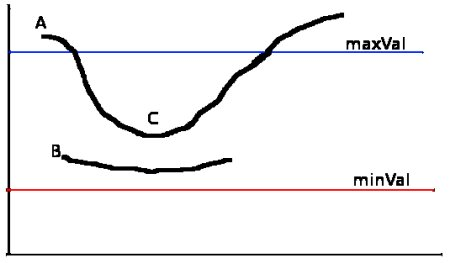
\includegraphics[width=0.5\textwidth]{2.png}
    \caption{\centering Histerezis prag}
\end{figure} 
\begin{figure}[h!]
    \centering
    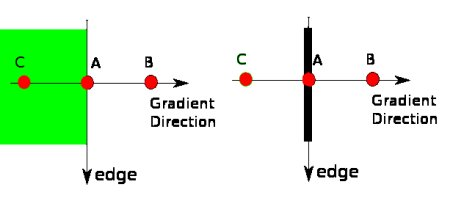
\includegraphics[width=0.5\textwidth]{1.png}
    \caption{\centering Nemaksimizujuće potiskivanje}
\end{figure} 

Po izostanku povezanosti ivica u implementaciji 5. se vrši povezivanje istih. Ivice će postati podebljanije i vidljivije. Obrada koja će se se obaviti je morfologička na osnovu oblika, uz primenu strukturoloških elemenata, tj. funkcija \verb|dilation|\cite{dilation}. Parametri su redom, ulazna slika, velicina kernela naspram kog je obavljena konvolucija, a dimenzije moraju biti neparne. Uvećava oblast beline na slici ili veličinu prvog plana slike, dat je primer na slici 3. i 4.

\begin{lstlisting}[language=Python, caption=Povezivanja i podebljivanje ivica]
    dilated = cv2.dilate(canny, (1, 1), iterations=0) 
    plt.imshow(dilated, cmap='gray') 
\end{lstlisting}

\begin{figure}[tbp!]
    \centering
    \begin{minipage}[b]{0.25\textwidth}
        
\includegraphics[width=1\textwidth]{3.png}
        \caption{\centering Početna slika}
    \end{minipage}
    % \hfill
    \begin{minipage}[b]{0.25\textwidth}
        
\includegraphics[width=1\textwidth]{4.png}
        \caption{\centering Izlazna slika nakon \texttt{dilation}-a}
    \end{minipage}
\end{figure}  

U implementaciji 6. nalaze se konture na slici \verb|cv2| funkcijom \verb|findContours|.\cite{findContours} Kontura važi za liniju koja spaja sve tačke kroz granice slike koje imaju isti intenzitet (tačaka). Najbolje je primenljiva nad slikama binarnih boja, tako da prethodno odrađeno detektovanje ivica je bilo delotvorno. Parametri koji su zastupljeni:
\begin{enumerate}
    \item ulazna slika - gde je urađeno duboko kopiranje;
    \item režim prihvatanja kontura - vrednost je \verb|RETR_EXTERNAL| - što daje spoljašnje konture\cite{retr};
    \item režim aproksimiranja kontura - kojom se čuvaju (x,y) koordinate granica oblika tačaka istih intenziteta. Ali ovime je ustanovljeno da li se baš sve tačke čuvaju ovim metodom. Vrednost je \verb|CHAIN_APPROX_NONE|, kojom se naznačava da se sve tačke konture čuvaju.
\end{enumerate}
A, višestruke povratne vrednosti koje su zastupljene:
\begin{enumerate}
    \item izlazna slika (ali ovde je zanemarena);
    \item konture;
    \item hijerarhija.
\end{enumerate}

Slika se iz BGR režima pretvara u RGB režim sačuvana u \verb|rgb| promenljivu. 

Iscrtavaju se konture sa funkcijom \verb|drawContours| kojoj su prosleđene slika,\cite{drawContours} konture, vrednost \verb|-1| koja označava da se iscrtavaju sve konture, torka elemenata domena [0, 255] RGB režima boja za svaki kanal i vrednost \verb|2| za debljinu iscrtane konture.
    
\begin{lstlisting}[language=Python, caption={Spajanje kontura, isticanje kontura na slici, plotovanje novonastale slikeħ}]
    (cnt, hierarchy) = cv2.findContours( 
    dilated.copy(), cv2.RETR_EXTERNAL, cv2.CHAIN_APPROX_NONE) 
    rgb = cv2.cvtColor(image, cv2.COLOR_BGR2RGB) 
    cv2.drawContours(rgb, cnt, -1, (255, 0, 0), 2) 
    
    plt.imshow(rgb) 
\end{lstlisting}
    
U implementaciji 7. ispisuje se brojnost kontura.

\begin{lstlisting}[language=Python, caption={Ispis broja kontura}]
    print("coins in the image : ", len(cnt)) 
\end{lstlisting}
%%%%%%%%%%%%%%%%%%%%%%%%%%%%%%%%%%%%%%%%%%%%%%%%%%%%%%%%%%%%%%%%%%%%%%%%%%%%%%%%%%%%%%%%%%%%
\subsection*{Drugi program - prebrojavanje boja}
U implementaciji 8. koristiće se \verb|numpy| i \verb|cv2| biblioteke.\cite{colonies}

\begin{lstlisting}[language=Python, caption={Uključivanje biblioteka}]
    # import the necessary packages
    import numpy as np
    import cv2
\end{lstlisting}

U implementaciji 9. priprema se rečnik \verb|counter| koji će se koristiti za prebrojavanje elemenata.

\begin{lstlisting}[language=Python, caption={Iniciranje rečnikom}]
    # dict to count colonies
    counter = {}
\end{lstlisting}

U implementaciji 10. vrši se učitavanje slike, a zatim se izvlače visina i širina slike.

\begin{lstlisting}[language=Python, caption={Učitavanje slike}]
    # load the image
    image_orig = cv2.imread("kondenzatori.jpg")
    height_orig, width_orig = image_orig.shape[:2]
\end{lstlisting}

U implementaciji 11. vrši se duboko kopiranje slike zarad kasnijeg generisanja slike sa konturama.
\begin{lstlisting}[language=Python, caption={Duboko kopiranje slike}]
    # output image with contours
    image_contours = image_orig.copy()
\end{lstlisting}

U implementaciji 12. definiše se lista elemenata vrednosti naziva boja koje će se detektovati, tj. plave i žute. Zatim se ostvaruje svaka iteracija pretlje po boji.

\begin{lstlisting}[language=Python, caption={Započeto iteriranje po bojama}]
    # DETECTING BLUE AND YELLOW CAPACITORS
    colors = ['blue', 'yellow']
    for color in colors:
\end{lstlisting}

U implementaciji 13. vrši se duboko kopiranje slike zarad neophodne međuobrade.

\begin{lstlisting}[language=Python, caption={Duboko kopiranje}]
    # copy of original image
    image_to_process = image_orig.copy()
\end{lstlisting}

U implementaciji 14. inicira se vrednost za ključ boje rečnika brojača na 0.

\begin{lstlisting}[language=Python, caption={Iniciranje odgovarajućeg ključa brojača}]
    # initializes counter
    counter[color] = 0
\end{lstlisting}
 
U implementaciji 15. na osnovu iteracije na osnovu boje definišu se BGR vektori boja za donju i gornju granicu boja koje se mogu uvažiti kao detektovana posmatrana boja.

\begin{lstlisting}[language=Python, caption={Nameštanje granica na osnovu boja}]
    # define NumPy arrays of color boundaries (GBR vectors)
    if color == 'blue':
        lower = np.array([ 60, 100,  20])
        upper = np.array([170, 255, 150])
    elif color == 'yellow':
        
        lower = np.array([ 50,  100,  100])
        upper = np.array([100, 255,  255])
\end{lstlisting}

U implementaciji 16. se proverava \verb|inRange|-om da li elementi liste leže između elemenata druge 2 liste, a broj elemenata određen zavisno od dimenzije. Po tome se određuje da li će pikselu kanal biti skroz zanemaren ili postavljen na maksimalnu vrednost, pa se sve to smesti u \verb|image_mask|, u vidu bitovske maske.\cite{inRange} Potom se proverava da li maska 1 bajta je nenula vrednost, ako jeste onda se uvažava izračunata konjunkcija bajtova između 2 prosleđene slike.\cite{konjunkcija}

\begin{lstlisting}[language=Python, caption={Bitovsko maskiranje i konjunkcije obavljene nad slikom}]
    # find the colors within the specified boundaries
    image_mask = cv2.inRange(image_to_process, lower, upper)
    # apply the mask
    image_res = cv2.bitwise_and(image_to_process, image_to_process, mask = image_mask)
\end{lstlisting} 

U implementaciji 17. se vrši konverzija iz BGR režima u grayscale \verb|cvtColor|-om, pa se potom vrši zamagljivanje uz \verb|GaussianBlur| gde je velicina Gausovog kernela \verb|(5,5)|, a standardna devijacija na obe ose postavljena je na \texttt{0}.

\begin{lstlisting}[language=Python, caption={Prosivljivanje i zamagljivanje slike}]
    ## load the image, convert it to grayscale, and blur it slightly
    image_gray = cv2.cvtColor(image_res, cv2.COLOR_BGR2GRAY)
    image_gray = cv2.GaussianBlur(image_gray, (5,5), 0)
\end{lstlisting} 

U implementaciji 18. vrši se prepoznavanje ivica uz \verb|Canny| i njihovo poboljšavanje \verb|dilate|-om u 1 iteraciji. Erozija je primenjena računanjem lokalnog minimuma (za razliku od \texttt{dilation}-a) nad oblašću zadatog kernel-a. Sada ivice bivaju tanje gde može se videti na slici 5 i 6. Uz ovu kombinaciju prvo se podebljanije vrši da bi se dobio efekat spajanja svih ivica, tako da nema prekida, a onda se istanjuju novodobijene ivice.

\begin{lstlisting}[language=Python, caption={Detekcija ivica i njihova obrada}]
    # perform edge detection, then perform a dilation + erosion to close gaps in between object edges
    image_edged = cv2.Canny(image_gray, 50, 100)
    image_edged = cv2.dilate(image_edged, None, iterations=1)
    image_edged = cv2.erode(image_edged, None, iterations=1)
\end{lstlisting} 

\begin{figure}[tbp!]
    \centering
    \begin{minipage}[b]{0.25\textwidth}
        
\includegraphics[width=1\textwidth]{3.png}
        \caption{\centering Početna slika}
    \end{minipage}
    % \hfill
    \begin{minipage}[b]{0.25\textwidth}
        
\includegraphics[width=1\textwidth]{5.png}
        \caption{\centering Izlazna slika nakon \texttt{erode}-a}
    \end{minipage}
\end{figure}  

Pronalaze se konture uz \verb|findContours| u implementaciji 19. samo što za razliku od prvog programa ovde se izvlače tačke po režimu metoda aproksimiranja samo one krajnje ako je u pitanju prava linija, inače kao i uvek sve tačke se uzimaju u obzir. Zatim se uzima prvi element liste koja je dobijena ovom funkcijom.

\begin{lstlisting}[language=Python, caption={Detekcija kontura}]
    # find contours in the edge map
    cnts = cv2.findContours(image_edged.copy(), cv2.RETR_EXTERNAL, cv2.CHAIN_APPROX_SIMPLE)[0]
\end{lstlisting} 

Ulazi se u ugnježdenu petlju u glavnoj petlji koja iterira kroz konture u implementaciji 20.

\begin{lstlisting}[language=Python, caption={Započeto iteriranje}]
    # loop over the contours individually
    for c in cnts:
\end{lstlisting} 

Proverava se da li ima dovoljno kontura neophodnih za uzimanje u obzir u implementaciji 21.

\begin{lstlisting}[language=Python, caption={Ispitivanje kriterijuma dovoljnosti brojnosti kontura}]
    # if the contour is not sufficiently large, ignore it
    if cv2.contourArea(c) < 5:
        continue
\end{lstlisting} 

Određuje se konveksna poleđina konture, tj. zove se \verb|cv2| funkcija \verb|convexHull| u implementaciji 22.

\begin{lstlisting}[language=Python, caption={Računanje konveksnih poleđina}]
    # compute the Convex Hull of the contour
    
    hull = cv2.convexHull(c)
\end{lstlisting} 

U implementaciji 23. će se iscrtati konture \verb|drawContours|-om, prosleđena je slika, lista u kojoj je samo jedan element promenljiva \verb|hull|, iscrtava se nulta kontura pošto je prosleđena \verb|0| za identifikator. Za plavu boju se iscrtava crvena kontura, a za žutu zelena, debljina konture će biti \verb|1|. Ovde se ugnježdena petlja koja iterira kroz konture završava.

\begin{lstlisting}[language=Python, caption={Iscrtavanje kontura na osnovu boja}]
            if color == 'blue':
    # 			prints contours in red color
                cv2.drawContours(image_contours,[hull],0,(0,0,255),1)
            elif color == 'yellow':
                # prints contours in green color
                cv2.drawContours(image_contours,[hull],0,(0,255,0),1)
\end{lstlisting} 

U implementaciji 24. se za boju brojač inkrementira za 1.
I tu se završava petlja koja iterira kroz boje.

\begin{lstlisting}[language=Python, caption={Ispis broja kontura po boji}]     
    counter[color] += 1
    # Print the number of capacitors of each color
    print("{} {} capacitors".format(counter[color],color))
\end{lstlisting} 

U implementaciji 25. se izlazna slika sa svim konturama iscrtanim ubacuje u datoteku \texttt{out.png}.

\begin{lstlisting}[language=Python, caption={Izbacivanje fajla rezultujuće slike}]     
    # Writes the output image
    cv2.imwrite("out.png",image_contours)
\end{lstlisting}

\subsection*{Treći program}
U implementaciji 26. sve na početku se vrši kao i u prvom programu, navođenje biblioteka i uključivanje slike iz zadatog fajla, sa grayscale bojama.\cite{stackoverfloweg}
\begin{lstlisting}[language=Python, caption={Učitavanje modula, učitavanje fajla slike}]     
import numpy as np
import cv2
img = cv2.imread("sp4.jpg", 0)
\end{lstlisting}

U implementaciji 27. se \verb|fastNlMeansDenoising|-om vrši odšumljivanje koristeći se algoritmom nelokalizujućih središta sa nekolicinom sračunljivih optimizacija. Šum se očekuje da bude Gausovog belog šuma. Očekuje se da se radi sa grayscale slikama.\cite{denoise} Implicitno se postavljaju parametri:
\begin{itemize}
    \item prozora pretrage \verb|search_window| sa vrednošću \verb|21| - gde se određuje veličina po pikselima prozora kojim će se računati prosečna težina piksela posebno, neparna je vrednost, linearno utiče na performanse.
    \item veličina bloka sa vrednošću \verb|7| - veličina po pikselima šablona zakrpe kojim se računaju težine, neparna.
\end{itemize}

Metod je zasnovan na jednostavnom principu, zamena boja piksela sa prosečno zastupljenom bojom sličnih piksela. Ali, od najuobičajenijih piksela do posmatranog piksela nemaju potrebe biti bliski. Dozvoljeno je skenirati poveći deo slike pri pretrazi naspram svih piksela koji se stvarno razaznaju naspram piksela koji će biti odšumljivan.\cite{denoise2}

\begin{lstlisting}[language=Python, caption={Odšumljivanje}]     
    # Denoising
denoisedImg = cv2.fastNlMeansDenoising(img);
\end{lstlisting}


U implementaciji 28. zove se \verb|cv2|-ova \verb|threshold| funkcija.\cite{tresh} Postavljaju se argumenti ranije obrađivana slika, prag, maksimalna vrednost koja će se kombinovati sa režimima definisanim \verb|THRESH_BINARY| i \verb|THRESH_BINARY_INV| (obrnut uslov anuliranja i postavljanja maksimalne vrednosti piksela), i flegovi \verb|THRESH_BINARY_INV| i \verb|THRESH_OTSU| popaljeni bitskom disjunkcijom.

Za svaki piksel primenjuje se isti prag. Ako vrednost piksela je manja od praga, ona se anulira. Inače, postavlja se na korisnički postavljenu maksimalnu vrednost. Slika koja se prosleđuje u funkciju mora biti grayscale.


Po globalnom usklađivanju pragom, koristi se arbitrarno izabrana vrednost kao prag. Nasuprot tome, \textbf{Otsu-ov metod} koji zaobilazi biranje vrednosti i određuje ga automatski. Uzima se u obzir slika sa samo 2 vrednosti piksela slike (binarna boja), gde histogram biva sastojan od samo 2 amplitude. Prag je određen tako da minimizuje težine disperzije unutar klasa.

$$
\sigma_w^2(t) = q_1(t)\sigma_1^2(t)+q_2(t)\sigma_2^2(t)
$$

$$
q_1(t) = \sum_{i=1}^{t} P(i) \quad \& \quad q_2(t) = \sum_{i=t+1}^{I} P(i)
$$

$$
\mu_1(t) = \sum_{i=1}^{t} \frac{iP(i)}{q_1(t)} \quad \& \quad \mu_2(t) = \sum_{i=t+1}^{I} \frac{iP(i)}{q_2(t)}
$$

$$
\sigma_1^2(t) = \sum_{i=1}^{t} [i-\mu_1(t)]^2 \frac{P(i)}{q_1(t)} \quad \& \quad \sigma_2^2(t) = \sum_{i=t+1}^{I} [i-\mu_2(t)]^2 \frac{P(i)}{q_2(t)}
$$

Sve je to odrađeno tako da vrednost $t$ koja leži na oblasti među dveju amplituda tako da disperzija obe klase je minimalna.

Dobar prag može biti sredina dveju vrednosti. I ovim metodom određen je optimalan globalni prag kao vrednost uz pomoć histograma.

\begin{lstlisting}[language=Python, caption={Nameštanje praga}]     
th, threshedImg = cv2.threshold(denoisedImg, 200, 255,cv2.THRESH_BINARY_INV|cv2.THRESH_OTSU) # src, thresh, maxval, type
\end{lstlisting}

U implementaciji 29. funkcija \verb|getStructuringElement| sa sobom definiše struktuirajući element, tj. kernel kojim se ističu režim (morfološki oblik \verb|MORPH_ELLIPSE| - elipsa upisana u pravougaonik \verb|Rect(0, 0, esize.width, 0, esize.height)|, pošto izričito radi sa kružno oblikovanim kernelima) i dimenzija.\cite{morphOps}\cite{mshape}

% https://docs.opencv.org/4.x/d4/d86/group__imgproc__filter.html#ga67493776e3ad1a3df63883829375201f

% src	Source image. The number of channels can be arbitrary. The depth should be one of CV_8U, CV_16U, CV_16S, CV_32F or CV_64F.
\verb|morphologyEx|-om obavljene su morfologičke transformacije korišćene \texttt{erosion} i \verb|dilation| kao osnovne operacije.\cite{mex} Bilo koja operacija može biti obavljena \textit{u mestu}. U slučaju više kanalnih slika, svaki kanal je procesuiran posebno nezavisno. Parametri koji su uzeti u obzir su:
\begin{enumerate}
    \item src - ulazna slika, broj kanala je arbitraran. Dubina može biti jedan od tipova, unsigned tipova kojima se ističe koliko memorije će zauzeti piksel, \verb|cv| modula;
    % op	Type of a morphological operation, see MorphTypes
    \item morfologička operacija tip, postavljena na \verb|MORPH_OPEN|, pa npr. po njoj će se operacije obavljati redosledom: \verb|erode -> erode -> dilate -> dilate|, ako ima 2 iteracije. Korisno je za uklanjanje šumova, kao na slici 6;
    % kernel	Structuring element. It can be created using getStructuringElement.
    \item kernel - preuzet od povratne vrednosti  \verb|getStructuringElement|-a;
    % anchor	Anchor position with the kernel. Negative values mean that the anchor is at the kernel center.
    \item  anchor - usidrena pozicija sa kernelom, negativnom vrednošću se naznačava da usidrenje je kernelov centar, implicitna vrednost koja se daje je \verb|(-1, -1)|;
    % iterations	Number of times erosion and dilation are applied.
    \item iterations - broj iteracija ponavljanja primene erosion i dilation operacija, implicitno je vrednost 1;
    \item borderType - vrednost granice u slučaju konstantne granice. Implicitno je \verb|BORDER_CONSTANT|, što naznačava kako se vrši zagraničavanje po šablonu \texttt{iiiiii|abcdefgh|iiiiiii}, gde naznačavaju se granice \texttt{|}, \texttt{i} je korisnički definisano. \verb|BORDER_WRAP| nije podržan;
    % borderValue	Border value in case of a constant border. The default value has a special meaning. 
    \item borderValue - gore pomenuto \texttt{i} - implicitno se radi na specijalan ``magičan'' način.
\end{enumerate}

\begin{lstlisting}[language=Python, caption={morfologičke operacije}]     
    kernel = cv2.getStructuringElement(cv2.MORPH_ELLIPSE, (5,5))
    morphImg = cv2.morphologyEx(threshedImg, cv2.MORPH_OPEN, kernel)
\end{lstlisting}

Na slici 7. može se videti primer ishoda morfološke operacije.

\begin{figure}[h!]
    \centering
    
\includegraphics[width=0.25\textwidth]{6.png}
    \caption{\centering Morfološka operacija \textit{opening}}
\end{figure} 


\begin{figure}[h!]
    \centering
    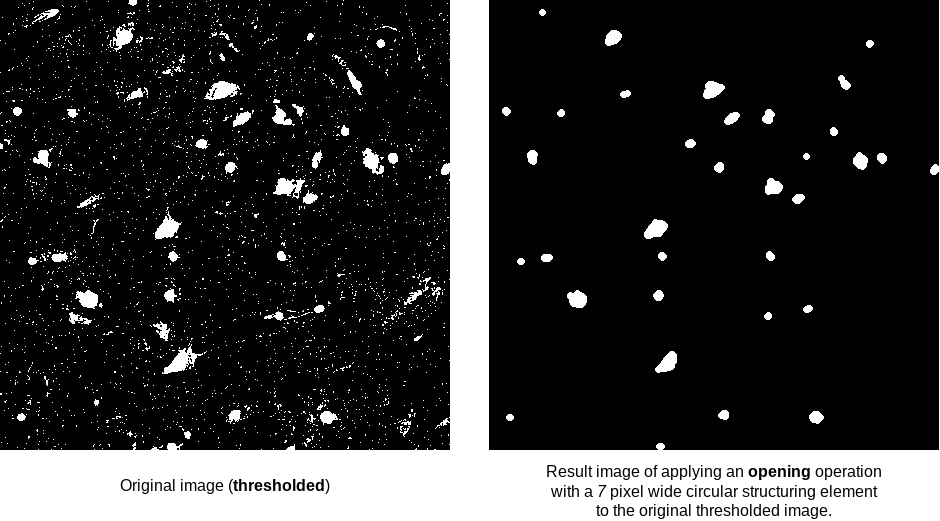
\includegraphics[width=0.75\textwidth]{7.png}
    \caption{\centering Morfološke operacije}
\end{figure} 

U implementaciji 30. koristi se \verb|findContours|, gde prihvata prethodno obrađenu sliku, drugi argument režim prihvatanja kontura \texttt{RETR\_TREE} (kojom se računa puna hijerarhija kontura), a uz \verb|CHAIN_APPROX_SIMPLE| izvlače tačke po režimu metoda aproksimiranja samo one krajnje ako je u pitanju prava linija, inače kao i uvek sve tačke se uzimaju u obzir.
\verb|cvtColor| vrši konverziju \texttt{GRAY2RGB} iz grayscale-a u RGB režim boja.
\verb|drawContours| kojoj su prosleđene slika, konture, vrednost \verb|-1| koja označava da se iscrtavaju sve konture, torka elemenata domena [0, 255] RGB režima boja za svaki kanal (u ovom slučaju plava) i vrednost \verb|3| za debljinu iscrtane konture.
\verb|imwrite|-om dostavlja se fajl slike \verb|_result.jpg| na odgovarajuću putanju.
Kasnije se ispisuje broj kontura u tekstualni fajl \verb|result.txt|, kojim se obgrljeno rezerviše tok fajla i razrešava tok resursa.

\begin{lstlisting}[language=Python, caption={Nalaze se konture, konverzija boja, crtanje kontura, dostavljanje izlaznog fajla slike, ispis broja kontura}]     
    # Find and draw contours
contours, hierarchy = cv2.findContours(morphImg, cv2.RETR_TREE, cv2.CHAIN_APPROX_SIMPLE)
contoursImg = cv2.cvtColor(morphImg, cv2.COLOR_GRAY2RGB)
cv2.drawContours(contoursImg, contours, -1, (0,0,255), 3)

cv2.imwrite("_result.jpg", contoursImg)
textFile = open("results.txt","a")
textFile.write("_result.jpg" + " Dots number: {}".format(len(contours)) + "\n")
print("Dots number: {}".format(len(contours)))
textFile.close()
\end{lstlisting}
\newpage
%%%%%%%%%%%%%%%%%%%%%%%%%%%%%%%%%%%%%%%%%%%%%%%%%%%%%%%%%%%%%%%%%%%%%%%%%%%%%%%%%%%

\renewcommand\lstlistingname{Izlaz}
\renewcommand\lstlistlistingname{Izlaz}
\setcounter{lstlisting}{0}

\section{Rezultati koda}
Biće izloženo obradi 4 slike 9., 10., 11., 12. štampanih ploča i slika kondenzatora 13., pa potom će se obaviti iscrtavanje kontura i prebrojavanje istih.
\begin{figure}[hbp!]
    \centering
    \begin{minipage}[b]{0.2\textwidth}
        
\includegraphics[width=1\textwidth]{u1.png}
        \caption{\centering 1. originalna slika štampane ploče}
    \end{minipage}
    % \hfill
    \begin{minipage}[b]{0.2\textwidth}
        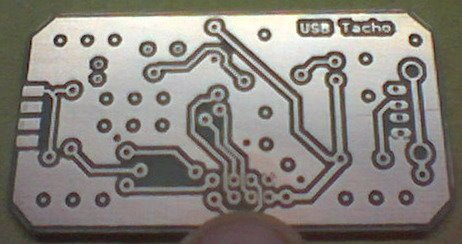
\includegraphics[width=1\textwidth]{u2.png}
        \caption{\centering  2. originalna slika štampane ploče}
    \end{minipage}
    \begin{minipage}[b]{0.2\textwidth}
        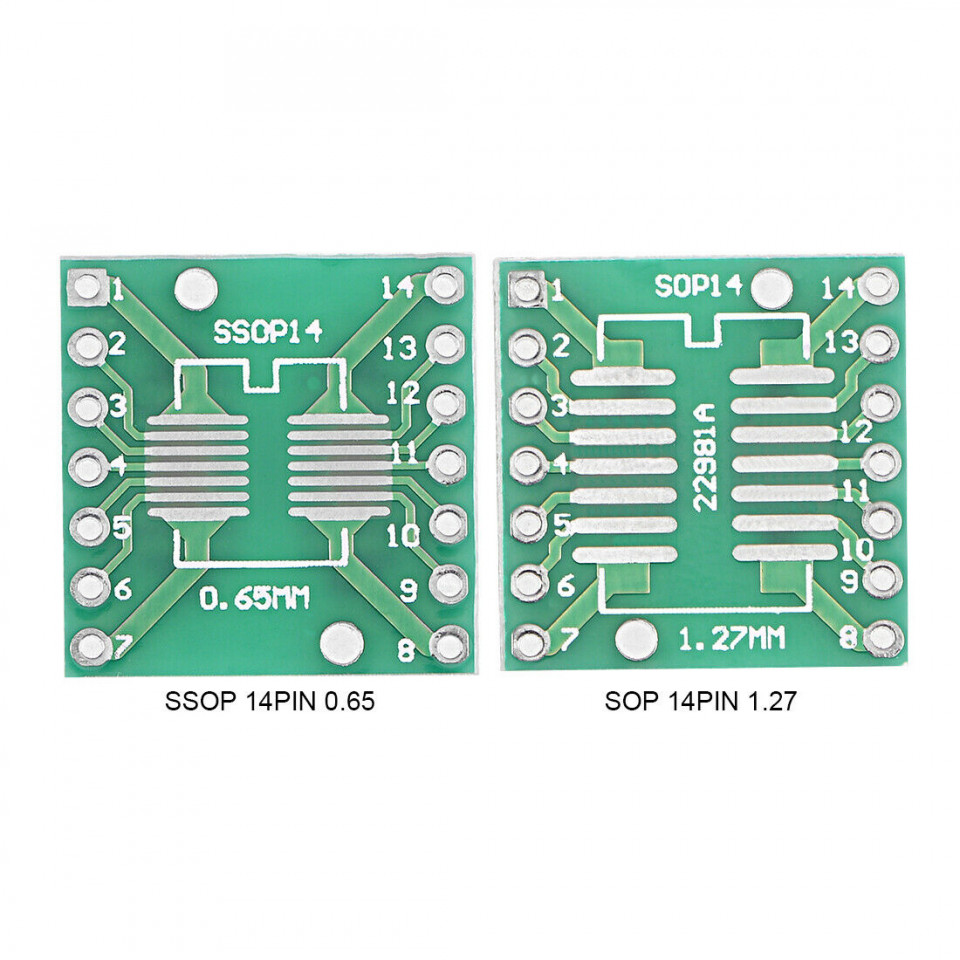
\includegraphics[width=1\textwidth]{u3.png}
        \caption{\centering  3. originalna slika štampane ploče}
    \end{minipage}
    \begin{minipage}[b]{0.2\textwidth}
        
\includegraphics[width=1\textwidth]{u4.png}
        \caption{\centering 4. originalna slika štampane ploče }
    \end{minipage}
    \begin{minipage}[b]{0.2\textwidth}
        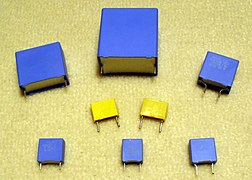
\includegraphics[width=1\textwidth]{u5.png}
        \caption{\centering Slika konderzatora}
    \end{minipage}
\end{figure}  
\newpage
\subsection*{Prvi program}

Cilj je obuhvatiti konturama vodove i konektore. Slika 14. prikazuje crvene konture koje su nađene za 1. originalnu sliku štampane ploče. A na izlazu 1. se ističe da je nađeno 526 kontura. 
\begin{figure}[h!]
    \centering
    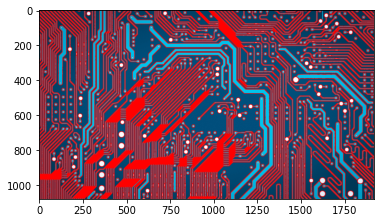
\includegraphics[width=0.5\textwidth]{11.png}
    \caption{\centering 1. program sa 1. slikom}
\end{figure} 

\begin{lstlisting}[caption=1. program sa 1. slikom]
    coins in the image :  526
\end{lstlisting}

Slika 15. prikazuje crvene konture koje su nađene za 2. originalnu sliku štampane ploče. A na izlazu 2. se ističe da je nađeno 48 kontura. 

\begin{figure}[h!]
    \centering
    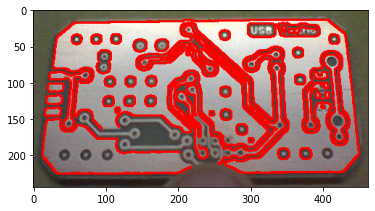
\includegraphics[width=0.5\textwidth]{12.png}
    \caption{\centering 1. program sa 2. slikom}
\end{figure} 

\begin{lstlisting}[caption=1. program sa 2. slikom]
coins in the image :  48
\end{lstlisting}
Slika 16. prikazuje crvene konture koje su nađene za 3. originalnu sliku štampane ploče. A na izlazu 3. se ističe da je nađeno 111 kontura. 
\begin{figure}[h!]
    \centering
    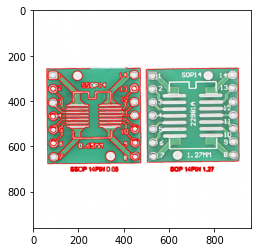
\includegraphics[width=0.5\textwidth]{13.png}
    \caption{\centering 1. program sa 3. slikom}
\end{figure} 

\begin{lstlisting}[caption=1. program sa 3. slikom]
coins in the image :  111
\end{lstlisting}

Slika 17. prikazuje crvene konture koje su nađene za 4. originalnu sliku štampane ploče. A na izlazu 4. se ističe da je nađeno 314 kontura. 

\begin{figure}[h!]
    \centering
    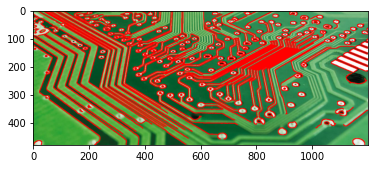
\includegraphics[width=0.5\textwidth]{14.png}
    \caption{\centering 1. program sa 4. slikom}
\end{figure} 

\begin{lstlisting}[caption=1. program sa 4. slikom]
coins in the image :  314
\end{lstlisting}

\subsection*{Drugi program}
Cilj je obuhvatiti konturama kondenzatore po bojama i prebrojati za svaku boju. Slika 18. prikazuje crvenom nagoveštava plava, a zelenom žuta. Na izlazu 5. ističe se da je obuhvaćeno 28 plavih kondenzatora, 13 žutih kondenzatora.

\begin{figure}[h!]
    \centering
    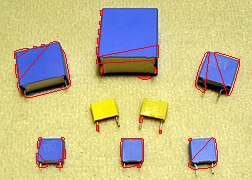
\includegraphics[width=0.5\textwidth]{21.png}
    \caption{\centering 2. program sa slikom plavih i žutih kondenzatora}
\end{figure} 

\begin{lstlisting}[caption=2. program sa slikom plavih i žutih kondenzatora]
28 blue capacitors
13 yellow capacitors
\end{lstlisting}

\subsection*{Treći program}

Cilj je isti kao i u prvo programu samo pristup je drugačiji, može se primetiti da pozadina slike binarne boje. Slika 19. prikazuje crvene konture koje su nađene za 1. originalnu sliku štampane ploče. A na izlazu 6. se ističe da je nađeno 441 kontura.

\begin{figure}[h!]
    \centering
    
\includegraphics[width=0.5\textwidth]{31.png}
    \caption{\centering 3. program sa 1. slikom}
\end{figure} 

\begin{lstlisting}[caption=3. program sa 1. slikom]
Dots number: 441
\end{lstlisting}

Slika 20. prikazuje crvene konture koje su nađene za 1. originalnu sliku štampane ploče. A na izlazu 6. se ističe da je nađeno 441 kontura.

\begin{figure}[h!]
    \centering
    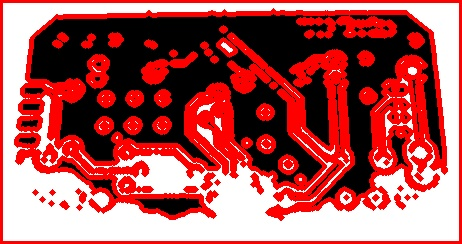
\includegraphics[width=0.5\textwidth]{32.png}
    \caption{\centering 3. program sa 2. slikom}
\end{figure} 

\begin{lstlisting}[caption=3. program sa 2. slikom]
Dots number: 227
\end{lstlisting}
Slika 21. prikazuje crvene konture koje su nađene za 2. originalnu sliku štampane ploče. A na izlazu 7. se ističe da je nađeno 227 kontura.
\begin{figure}[h!]
    \centering
    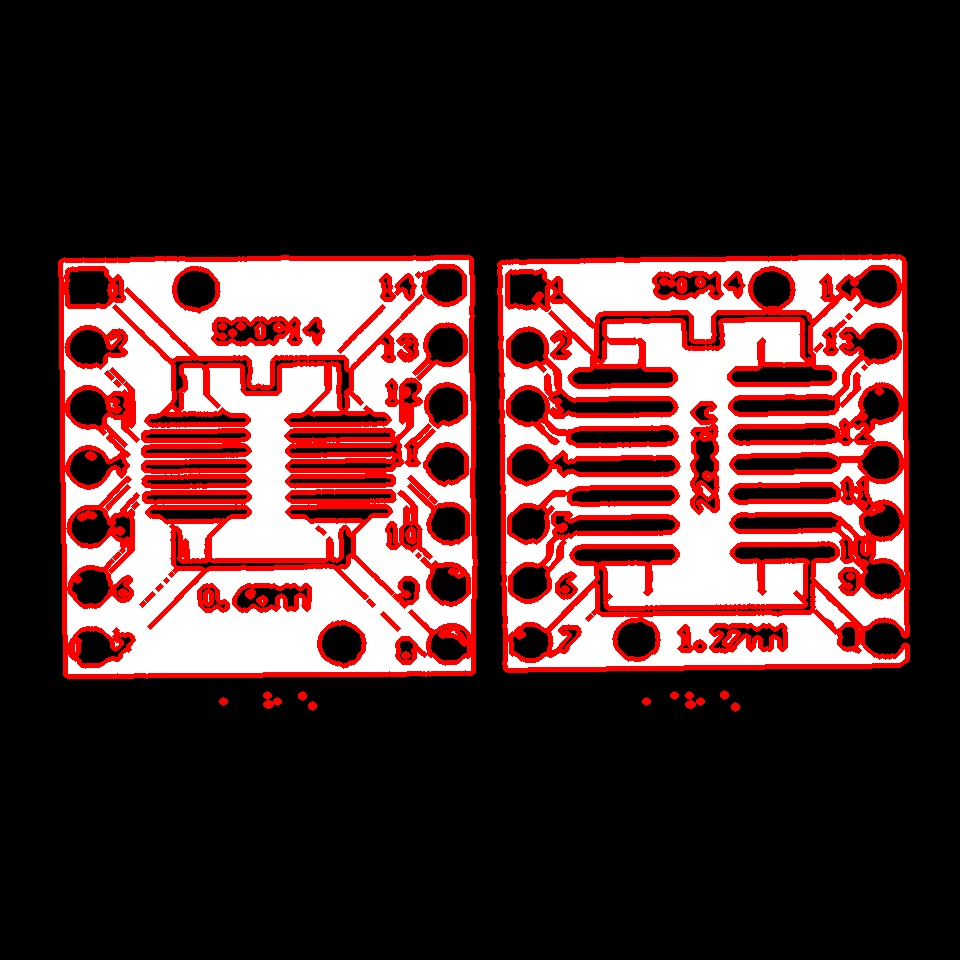
\includegraphics[width=0.35\textwidth]{33.png}
    \caption{\centering 3. program sa 3. slikom}
\end{figure} 

Slika 22. prikazuje crvene konture koje su nađene za 3. originalnu sliku štampane ploče. A na izlazu 8. se ističe da je nađeno 861 kontura.
\begin{lstlisting}[caption=3. program sa 3. slikom]
Dots number: 861
\end{lstlisting}

Slika 23. prikazuje crvene konture koje su nađene za 4. originalnu sliku štampane ploče. A na izlazu 9. se ističe da je nađeno 201 kontura.

\begin{figure}[h!]
    \centering
    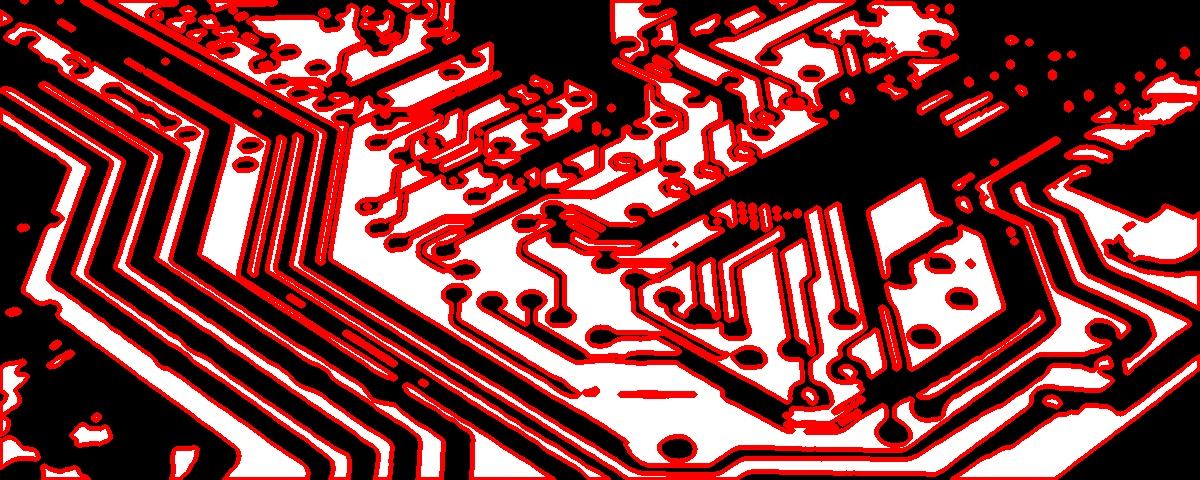
\includegraphics[width=0.5\textwidth]{34.png}
    \caption{\centering 3. program sa 4. slikom}
\end{figure} 
\begin{lstlisting}[caption=3. program sa 4. slikom]
Dots number: 201
\end{lstlisting}
%%%%%%%%%%%%%%%%%%%%%%%%%%%%%%%%%%%%%%%%%%%%%%%%%%%%%%%%%%%%%%%%%%%%%%%%%%%%%%%%%%%%%%%%%%%%
\newpage
\section{Zaključak}
Može se uočiti da se u sva tri programa koristile iste funkcije, ali poneki parametar za svaki program je bio zasebno služio kao jedinstven primer. 

U prvom programu se davao značaj na posivljivanju, zamaglivanju, detektovanju ivica, povezivanju i podebljavanju ivica, nalaženju kontura naspram ivica svih tačaka, krajnjoj konverziji u RGB, pa iscrtavanju kontura. 

Drugi program dao je značaj na detekciji boja uz definisanju gornjih i donjih ograničenja, radu sa maskama naspram tih granica, pa tek onda posivljivanju, \verb|dilate| funkciji, a sada eroziji, nalaženju kontura, ispitivanju dovoljnosti kontura, iscrtavanju i prebrojavanju kontura po bojama.

U trećem zadatku se davao značaj na definisanju praga, korisnički definisanim maksimalnim vrednostima definisanje ili anuliranje piksela, otsu režima ustanovljavanja pragova i detekcije ivica, rad sa \verb|dilate| i \verb|erosion| elipsom i njihovim redosledom izvšavanja zarad kranjeg rašumljavanja, pa se nalazile konture, iscrtavale i prebrojavale. 

Rezultati za sva tri programa su bili približni i naziralo se da su bili delotvorni, ali ne i previše pouzdani.

Po prvom programu deluje da je obuhvaćeno obradom većina poželjnih entiteta na koje se ciljalo, ali ima izostanaka. Po slici i po brojnosti, ali je to opet upitno.

Po drugom programu se nazire neka doslednost da ide u pravcu nekog razaznavanja entiteta, ali to nije savršeno i moguća nepogodnost je ta što nije dovoljno velika rezolucija, a i pozadina zavarava prebrojavanje žutih kondenzatora. Brojnost je više od pet puta veća, ali i verovatno da konture nisu dosledne tačnosti.

Po trećem programu vizuelna uočljivost prepoznatih entiteta kontura na slici je većinski poklopljena sa ciljanim stanjem, ali brojnostje mnogostruko veća i nepouzdana.

\newpage
\begin{thebibliography}{1}
    \bibitem{g4g}
    Count number of Object using Python-OpenCV,

    \url{https://www.geeksforgeeks.org/count-number-of-object-using-python-opencv/}, 
    
    Datum posete: \today

    \bibitem{canny}
    Canny Edge Detection,
    
    \url{https://docs.opencv.org/4.x/da/d22/tutorial_py_canny.html},
    
    Datum posete: \today

    \bibitem{dilation}
    Erosion and Dilation of images using OpenCV in python,

    \url{https://www.geeksforgeeks.org/erosion-dilation-images-using-opencv-python/}

    Datum posete: \today
    
    \bibitem{findContours}
    Find and Draw Contours using OpenCV | Python,

    \url{https://www.geeksforgeeks.org/find-and-draw-contours-using-opencv-python/},

    Datum posete: \today

    \bibitem{retr}
    difference between \verb|CV_RETR_LIST,CV_RETR_TREE,CV_RETR_EXTERNAL?|,

    \url{https://stackoverflow.com/questions/8830619/difference-between-cv-retr-list-cv-retr-tree-cv-retr-external},

    Datum posete: \today
    \bibitem{drawContours}
    Drawing Functions Image Processing, 

    \url{https://docs.opencv.org/4.x/d6/d6e/group__imgproc__draw.html#ga746c0625f1781f1ffc9056259103edbc}

    Datum posete: \today

    \bibitem{colonies}
    Counting blue and white bacteria colonies with Python and OpenCV,

    \url{http://www.sixthresearcher.com/counting-blue-and-white-bacteria-colonies-with-python-and-opencv/},

    Datum posete: \today
    \bibitem{inRange}
    Operations on arrays, Core functionality, inRange,

    \url{https://docs.opencv.org/3.4/d2/de8/group__core__array.html#ga48af0ab51e36436c5d04340e036ce981},

    Datum posete: \today
    \bibitem{konjunkcija}
    Operations on arrays, Core functionality, bitwise\_and,

    \url{https://docs.opencv.org/3.4/d2/de8/group__core__array.html#ga60b4d04b251ba5eb1392c34425497e14},

    Datum posete: \today
    \bibitem{stackoverfloweg}
    Count cells on image using python and OpenCV,

    \url{https://stackoverflow.com/questions/60957257/count-cells-on-image-using-python-and-opencv},

    Datum posete: \today
    \bibitem{denoise}
    fastNlMeansDenoising,

    \url{https://docs.opencv.org/3.4/d1/d79/group__photo__denoise.html},
    
    Datum posete: \today

    \bibitem{denoise2}
    A. Buades, B. Coll, J.M. Morel,  Non-Local Means Denoising (2011), IPOL Journal · Image Processing On Line,
    
    \url{http://www.ipol.im/pub/art/2011/bcm_nlm/},
    
    Datum posete: \today
    \bibitem{tresh}
    Image Thresholding,
    
    \url{https://docs.opencv.org/4.x/d7/d4d/tutorial_py_thresholding.html}

    Datum posete: \today
    \bibitem{morphOps}
    Morphological Transformations,

    \url{https://docs.opencv.org/4.x/d9/d61/tutorial_py_morphological_ops.html},

    Datum posete: \today
    \bibitem{mshape}
    MorphShapes,

    \url{https://docs.opencv.org/4.x/d4/d86/group__imgproc__filter.html#gac2db39b56866583a95a5680313c314ad}

    Datum posete: \today
    \bibitem{mex}
    morphologyEx,

    \url{https://docs.opencv.org/4.x/d4/d86/group__imgproc__filter.html#ga67493776e3ad1a3df63883829375201f},

    Datum posete: \today
\end{thebibliography}
\end{document}